\paragraph{}
Over this chapter, the \textbf{space communication protocols} are going to be defined. That is, a set of rules are going to be established in order to achieve the actual node-to-node communication. Altough the scope of the chapter is limited to the space segment, this inital introduction on the protocol definition is usfeul for the ground segment.
Having said that, several factors constrain the design of this relation of rules:

\begin{itemize}
\renewcommand{\labelitemi}{\scriptsize$\blacksquare$} 
\item \textbf{Speed:} As it has already been mentioned, each node should be capable of handling at least \textbf{25} Mbit/s. Even though this doesn't mean that the design should be able to fit 25 Mbit/s of pure costumer data, it is still a strong requirement with many effects over the system. For example, some protocols are just too slow establishing the connection; those will be directly discarded.

\item \textbf{Reliability:} The protocols have to assure that the messages are going to arrive to their destination. In order to achieve this, a routing protocol has to be used as well.


\item \textbf{Security:} Messages are not just required to arrive to their destination but they also must be ordered and coherent when they reach the client. That is the reason why error control is taken into consideration very seriously along the design process.
\end{itemize}
In the diagram \ref{fig:osi}, it can be clearly seen the structure of a protocol stack. Each layer has an underlying protocol, designed to achieve a specific task. There are \textbf{low-level} protocols, dealing with \textit{hardware} or with the establishment of the \textit{physical} path between two nodes. Also, there are the \textbf{high-level} protocols, dealing with session control, optimum \textit{logical} paths generation and bridging the application layer with the physical layer.
\begin{figure}[H]
\centering
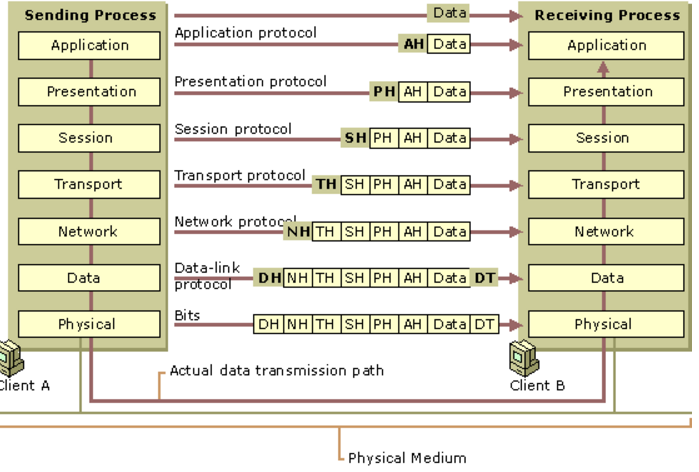
\includegraphics[scale=0.8]{./sections/CommunicationsDept/OSI}
\caption{OSI Model layers}
\label{fig:osi}
\end{figure}

As it can be deducted, both the sending and the receiving node have to work in coordination. Also, each layer is designed with encapsulation in mind. Therefore, each layer does not depend on the others and develops its own task independently.

This philosophy has been started by the \textit{International Telecommunications Unit} or \textbf{ITU} who first proposed, in the late 1970, the previously depicted \textbf{OSI Model}. Basiaclly, it establishes a conceptual framework for when new protocols are to be designed. Each layer can be understood easily if one thinks as the act of sending mail by post, for instance.

As far as \textit{Astrea constellation} is concerned, the physical layer is already defined in detail in the \textbf{Satellite Desgin} part. Since the\textbf{ Data Link layer}, the \textbf{Network layer} and the \textbf{Transport/Session layer} are of vital importance for the communication to work, the aim of the next sections will be to define the protocol that the constellation will be using for each one of those layers.

The presentation and the application layer are more client oreinted. In other words, if one client's satellite sends some data formatted with an unknown application protocol, \textit{Astrea} will not be affected in any way. What astrea will do is add to this stream of bits, some headers, in order for the message to arrive in time to its destination. This methodology is undoubtedly positive for \textit{Astrea} since the respobility of the application data will be solely for the customer.